\documentclass{beamer}
%\documentclass[handout]{beamer}

\mode<presentation>
{
  %\usetheme{CambridgeUS}
  %\usetheme{Frankfurt}
  \usetheme{Singapore}
  %\usecolortheme{crane}
  \usefonttheme{professionalfonts}
  %\usefonttheme[onlymath]{serif}
  
  \setbeamertemplate{blocks}[rounded][shadow=true]
}

\usepackage{pgfpages}

\usepackage{alltt,verbatim,amsmath,times,empheq}
\usepackage{bm}
\usepackage[english]{babel}
\usepackage[utf8]{inputenc}

%\usepackage{times}
%\usepackage[T1]{fontenc}
% Or whatever. Note that the encoding and the font should match. If T1
% does not look nice, try deleting the line with the fontenc.

%\usepackage{hyperref}

\usepackage{pdfanim}
\usepackage{multimedia,xmpmulti}

\PDFAnimLoad[width=\textwidth,loop,interval=40]{exp3a}{exp3a/pic}{310}%

\usepackage{animate}

\definecolor{dark red}{HTML}{E41A1C}
\definecolor{dark green}{HTML}{4DAF4A}
\definecolor{dark violet}{HTML}{984EA3}
\definecolor{dark blue}{HTML}{084594}
\definecolor{dark orange}{HTML}{FF7F00}
\definecolor{light blue}{HTML}{377EB8}
\definecolor{light red}{HTML}{FB9A99}
\definecolor{light violet}{HTML}{CAB2D6}

\setbeamercolor{boxed}{fg=black,bg=uaf yellow}

\newcommand{\CC}{\mathbb{C}}
\newcommand{\NN}{\mathbb{N}}
\newcommand{\RR}{\mathbb{R}}
\newcommand{\ZZ}{\mathbb{Z}}
\newcommand{\Acal}{\mathcal{A}}
\newcommand{\Bcal}{\mathcal{B}}
\newcommand{\Ccal}{\mathcal{C}}
\newcommand{\Ncal}{\mathcal{N}}
\newcommand{\Kcal}{\mathcal{K}}

\newcommand{\bF}{\mathbf{F}}
\newcommand{\bQ}{\mathbf{Q}}
\newcommand{\bU}{\mathbf{U}}
\newcommand{\bbU}{\bar{\bU}}
\newcommand{\bu}{\mathbf{u}}
\newcommand{\bv}{\mathbf{v}}
\newcommand{\bx}{\mathbf{x}}

\newcommand{\Div}{\nabla\cdot}
\newcommand{\eps}{\epsilon}
\newcommand{\grad}{\nabla}
\newcommand{\lap}{\triangle}
\DeclareMathOperator{\trace}{tr}
\renewcommand{\bar}{\overline}

\newcommand{\ddx}[1]{\frac{\partial #1}{\partial x}}
\newcommand{\ddy}[1]{\frac{\partial #1}{\partial y}}
\newcommand{\pp}[2]{\frac{\partial #1}{\partial #2}}
\newcommand{\ppt}[1]{\frac{\partial #1}{\partial t}}
\newcommand{\ppT}[1]{\frac{\partial #1}{\partial T}}
\newcommand{\ppx}[1]{\frac{\partial #1}{\partial x}}
\newcommand{\ppy}[1]{\frac{\partial #1}{\partial y}}
\newcommand{\ppz}[1]{\frac{\partial #1}{\partial z}}
\newcommand{\ppxx}[1]{\frac{\partial^2 #1}{\partial x^2}}
\newcommand{\ppzz}[1]{\frac{\partial^2 #1}{\partial z^2}}

\newcommand{\Tnorm}[1]{\left|\!\left|\!\left|#1\right|\!\right|\!\right|}
\newcommand{\rhow}{\rho_{\text{w}}}
\newcommand{\Wq}{W^{1,q}(\Omega)}
\newcommand{\half}{\frac12}

%\setbeamercolor{redtext}{fg=red!80!black}
\setbeamercolor{redtext}{fg=red!94!black}
%\setbeamercolor{greentext}{fg=green!80!black}
\setbeamercolor{greentext}{fg=green!60!black}
%\setbeamercolor{bluetext}{fg=blue!70!black}
\setbeamercolor{bluetext}{fg=blue!90!black}
\setbeamercolor{yellowtext}{fg=yellow!95!black}
\setbeamercolor{orangetext}{fg=yellow!50!red}

\newcommand{\green}{\usebeamercolor[fg]{greentext}}
\newcommand{\blue}{\usebeamercolor[fg]{bluetext}}
\newcommand{\red}{\usebeamercolor[fg]{redtext}}

\renewcommand{\L}{\emph{Left}}
\newcommand{\R}{\emph{Right}}



\title[weak and shallow ice sheet flows]{Weak and shallow: \\ New thinking about simulations of  \\ ice sheet flows}

\author[Bueler]{Ed Bueler}

\institute[UAF]{
  \tiny Dept of Mathematics and Statistics and Geophysical Institute \\

  University of Alaska Fairbanks
}

\date{\tiny 27 October, 2012}


\setbeamerfont{date}{size=\scriptsize}

\subject{ice sheet modelling, ice sheets, ice streams, numerical analysis, variational inequality}


%\begin{comment}
\AtBeginSection[]
{
  \begin{frame}<beamer>
    \frametitle{Outline}
    \tableofcontents[currentsection,hideallsubsections]
  \end{frame}
}
%\end{comment}


\begin{document}
\graphicspath{{figs/},{../commonfigs/},{photos/}}

\begin{frame}
  \titlepage
  \begin{center}
  \tiny supported by NASA grant NNX09AJ38C
  \end{center}
\end{frame}


\begin{frame}
  \frametitle{weak, shallow, and fairly new}

\begin{itemize}
\small
\item C.~Schoof (\textbf{2006}) \emph{A variational approach to ice stream flow}, J.~Fluid Mech.~556, 227--251
\medskip
\item E.~Bueler, J.~Brown (\textbf{2009}) \emph{Shallow shelf approximation as a “sliding law” in a thermodynamically coupled ice sheet model}, J.~Geophys.~Res.~114, F03008
\medskip
\item \alert<2>{G.~Jouvet}, E.~Bueler (\textbf{2012}) \emph{Steady, shallow ice sheets as obstacle problems: well-posedness and finite element approximation}, SIAM J.~Appl.~Math.~72 (4), 1292--1314
\medskip
\item \alert<2>{G.~Jouvet}, E.~Bueler, C.~Gr\"aser, R.~Kornhuber (\textbf{to appear})  \emph{A nonsmooth Newton multigrid method for a hybrid, shallow model of marine ice sheets}, Proc.~8th ICSCA, AMS Cont.~Math.
\end{itemize}

\small
\onslide<2>{\alert{G.~Jouvet} = Guillaume Jouvet, Free University of Berlin}
\end{frame}


% NO OUTLINE BECAUSE ONE APPEARS AT START OF EACH SECTION:
%\begin{comment}
\begin{frame}
  \frametitle{Outline}
  \tableofcontents[hideallsubsections]
  % You might wish to add the option [pausesections]
\end{frame}
%\end{comment}


\section[intro]{ice sheet flow: an introduction for non-glaciologists}


\begin{frame}{ice in glaciers is a viscous fluid}
\begin{columns}
\begin{column}{0.65\textwidth}
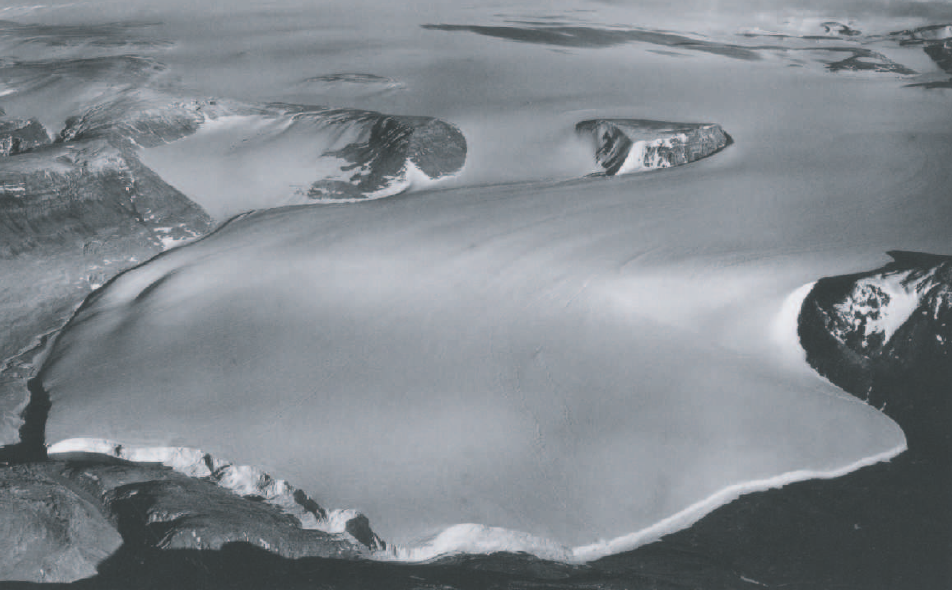
\includegraphics[width=1.0\textwidth]{polaris}
\end{column}
\begin{column}{0.35\textwidth}
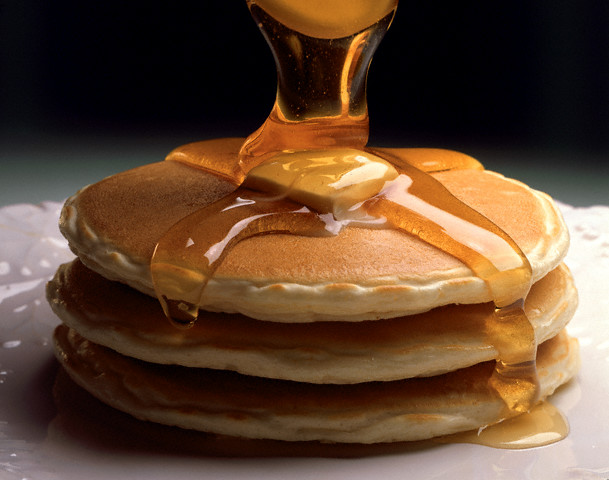
\includegraphics[width=1.0\textwidth]{pancakes}
\end{column}
\end{columns}

\bigskip\bigskip
\begin{itemize}
\item \dots at least: glaciers are viscous flows at larger scales
\item \emph{usage}: ``ice sheets'' are big, shallow glaciers
\end{itemize}
\end{frame}


\begin{frame}{ice in glaciers is a viscous fluid}

\begin{itemize}
\item primary variables: velocity $\mathbf{u}(\bx,t)$ and pressure $p(\bx,t)$
\item also: $\rho$ is density, $\mathbf{g}$ is gravity, $\nu$ is viscosity
\item if the glacier fluid were ``typical'' like the ocean we would model with Navier-Stokes equations:
\begin{align*}
\nabla \cdot \mathbf{u} &= 0 &&\text{\emph{incompressibility}} \\
\rho \left(\mathbf{u}_t + \mathbf{u}\cdot\nabla \mathbf{u}\right) &= -\nabla p + \nu \nabla^2 \mathbf{u} + \rho \mathbf{g} &&\text{\emph{stress balance}}
\end{align*}
\item but ice is not typical!
\item e.g.~not addressed in ice sheet flow models:
  \begin{itemize}
  \item[$\circ$] turbulence
  \item[$\circ$] convection
  \item[$\circ$] coriolis force
  \item[$\circ$] density-driven flow
  \end{itemize}
\end{itemize}
\end{frame}


\begin{frame}{ice is a slow, shear-thinning viscous fluid}

\begin{itemize}
\item our glacier fluid is
  \begin{enumerate}
  \item ``slow''\footnote{$Fr\approx 10^{-15}$.  Regarding coriolis: $Fr/Ro \approx 10^{-8}$.}:
    $$\rho \left(\mathbf{u}_t + \mathbf{u}\cdot\nabla \mathbf{u}\right) \approx 0 \qquad \iff \qquad \begin{pmatrix} \text{forces of inertia} \\ \text{are negligible} \end{pmatrix}$$
  \item non-Newtonian (shear-thinning):
    $$\text{viscosity $\nu$ is not constant}$$
  \end{enumerate}
\end{itemize}
\end{frame}


\begin{frame}{ice is a slow, shear-thinning viscous fluid}

\begin{itemize}
\item notation:
  \begin{itemize}
  \item[$\circ$] $\tau_{ij}$ is deviatoric stress tensor
  \item[$\circ$] $\mathbf{D}u_{ij}$ is strain rate tensor
  \end{itemize}
\smallskip
\item the standard ice flow model is Glen-law Stokes:
\begin{align*}
\nabla \cdot \mathbf{u} &= 0 &&\text{\emph{incompressibility}} \\
0 &= - \nabla p + \nabla \cdot \tau_{ij} + \rho \mathbf{g} &&\text{\emph{slow stress balance}} \\
\mathbf{D}u_{ij} &= A \left|\tau_{ij}\right|^{n-1} \tau_{ij} &&\text{\emph{Glen flow law}}
\end{align*}
\item $1.8 < n < 4.0$ ?  \quad \fbox{when in doubt: $n=3$}
\medskip
\item $A>0$ is called ``ice softness''
  \begin{itemize}
  \item[$\circ$] strongly $T$-dependent \dots but we'll not worry about that here
  \end{itemize}
\end{itemize}
\end{frame}


\begin{frame}{because ice is a slow fluid \dots}

\begin{itemize}
\item  geometry, boundary stress, and viscosity determine velocity field and pressure instantaneously (i.e.~in the Stokes model)

\bigskip
\item \emph{thus}: a time-stepping ice sheet code recomputes the velocity field at every time step, without requiring previous velocity \footnote{to be a weatherman you've got to know which way the wind blows \dots but not to be a glaciologist}
\end{itemize}
\end{frame}


\begin{frame}{ice sheets are ``shallow''}

\begin{itemize}
\item consider cross section of Greenland ice sheet at $71^\circ$ N
\small
  \begin{itemize}
  \item[$\circ$] {\color{dark green}{green}} and {\color{dark blue}{blue}}: usual vertically-exaggerated version
  \end{itemize}
  \begin{center}
    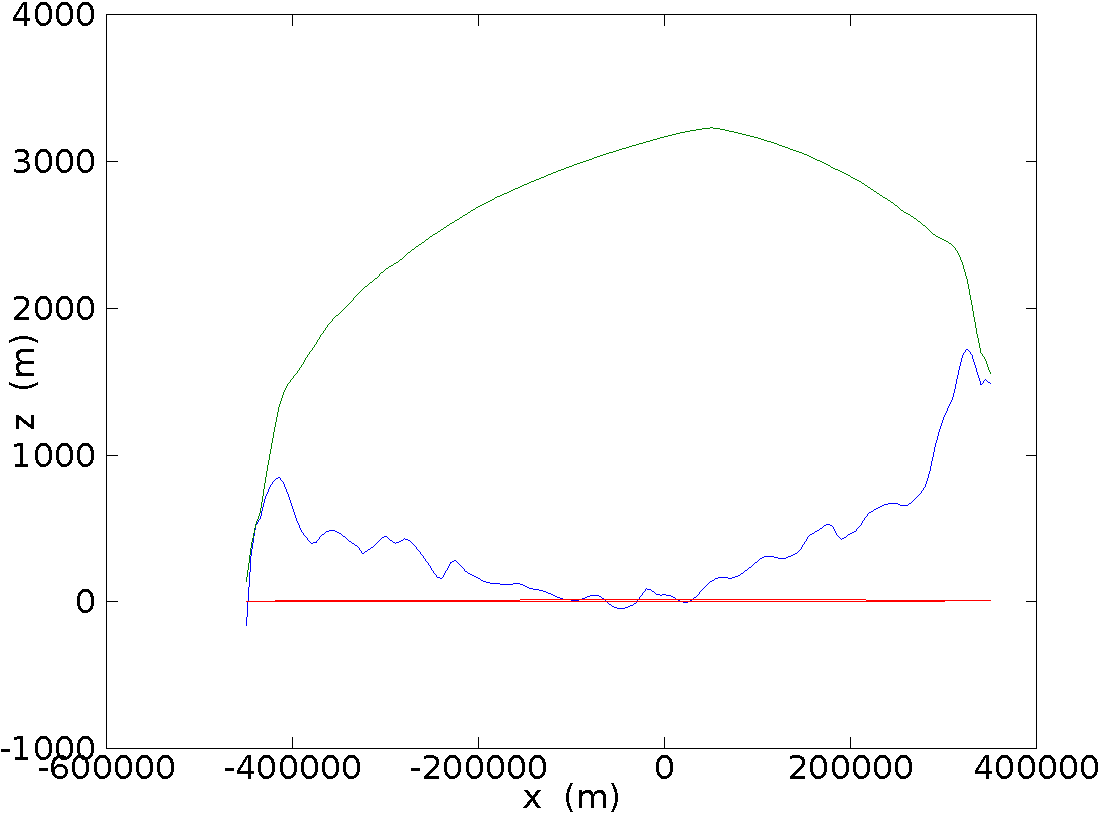
\includegraphics[width=0.5\textwidth]{greentrans}
  \end{center}
\normalsize
\item in {\color{dark red}{red}}: a view without this vertical exaggeration
\item \emph{thus}: 
  \begin{itemize}
  \item[$\circ$] most simulations use shallow limits of Stokes
  \item[$\circ$] high aspect-ratio elements endanger Stokes solvers
  \end{itemize}
\end{itemize}
\end{frame}


\begin{frame}{ice sheets versus ice shelves}

\begin{columns}
\begin{column}{0.35\textwidth}
\small
\begin{itemize}
\small
\item non-sliding portions of ice sheets flow by shear deformation
\item ice streams slide
\item ``ice shelves'' are floating thick ice
  \begin{itemize}
  \scriptsize
  \item[$\circ$] $\ne$ sea ice
  \end{itemize}
\item ice shelves flow by extension
  \begin{itemize}
  \scriptsize
  \item[$\circ$] ``membrane'' or ``plug'' flow
  \end{itemize}
\end{itemize}
\end{column}

\begin{column}{0.65\textwidth}
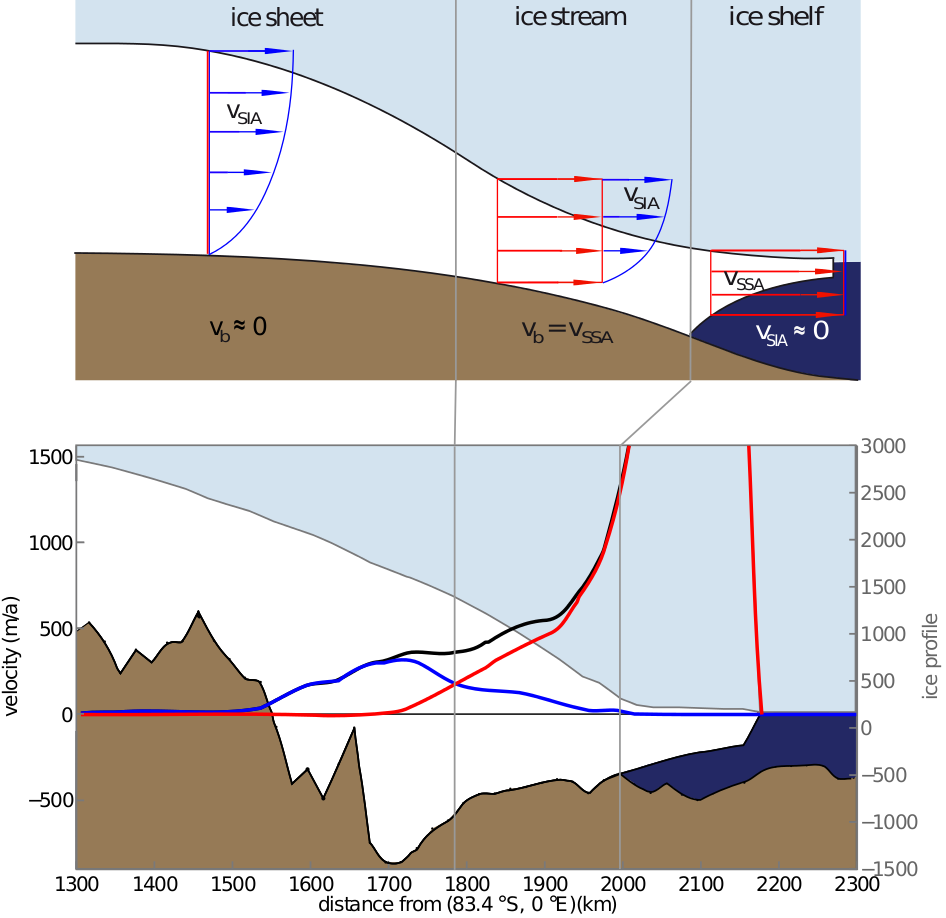
\includegraphics[width=\textwidth]{siassacartoon-lambert}

\begin{center}
\vspace{-0.18in}
\tiny [Lambert glacier and Amery ice shelf, Antarctic]
\end{center}
\end{column}
\end{columns}
\end{frame}


\begin{frame}{shear versus extension}

\begin{columns}
\begin{column}{0.35\textwidth}
\small
\begin{itemize}
\item \emph{top}:  non-sliding, sliding, and floating modes
\item \emph{bottom}:  real sheet-stream-shelf transition
\item ``SIA'' and ``SSA'' will be explained later
\end{itemize}
\end{column}

\begin{column}{0.65\textwidth}
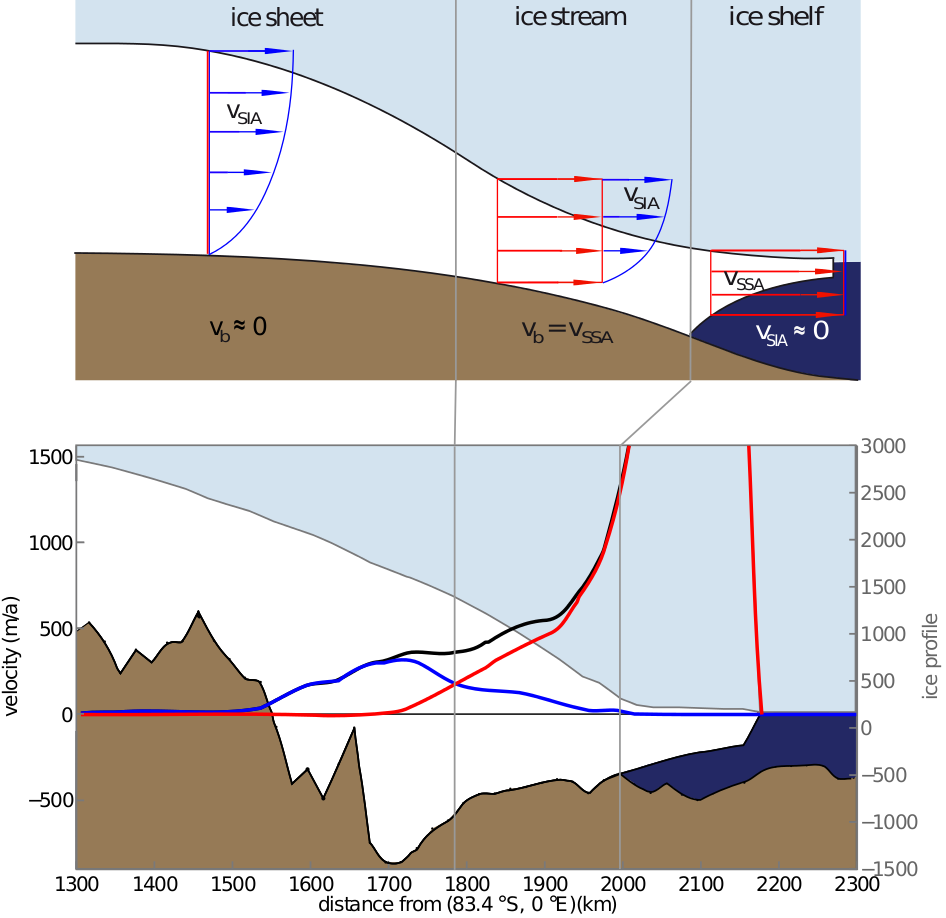
\includegraphics[width=\textwidth]{siassacartoon-lambert}

\begin{center}
\vspace{-0.18in}
\tiny [Lambert glacier and Amery ice shelf, Antarctic]
\end{center}
\end{column}
\end{columns}
\end{frame}


\begin{frame}{summary so far}

\begin{itemize}
\item ice sheets have four outstanding properties \emph{as viscous flows}:
  \begin{enumerate}
  \item \alert{slow}
  \item \alert{shear-thinning}
  \item \alert{shallow}
  \item \alert{contact slip}
  \end{enumerate}
\end{itemize}
\end{frame}


\begin{frame}
  \frametitle{big picture: ice sheet flow affects sea level}

\medskip
\small
if we think of an ice sheet as an input/output device:
\begin{itemize}
\item \emph{inputs}: (1) snow adds, (2) sun heats, (3) ocean heats, (4) earth heats
\item \emph{outputs}: (1) surface meltwater, (2) basal meltwater, (3) ice discharge
\end{itemize}

\begin{center}
  %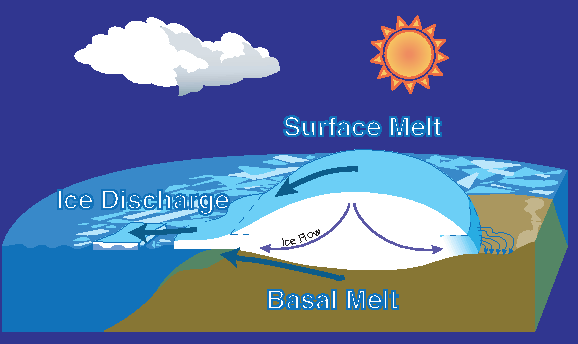
\includegraphics[width=0.7\textwidth]{ice-sheet-cartoon}
  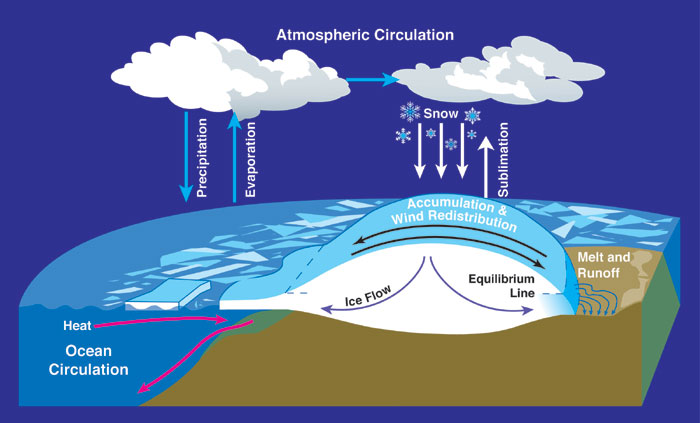
\includegraphics[width=0.75\textwidth]{mass-bal-atmos}

  %\tiny (figure from IceSAT brochure)
\end{center}
\end{frame}


\begin{frame}
  \frametitle{big picture: ice sheet flow changes over time}

\small
\begin{itemize}
\item boxes show estimates of mass loss rate from Greenland:
\begin{center}
    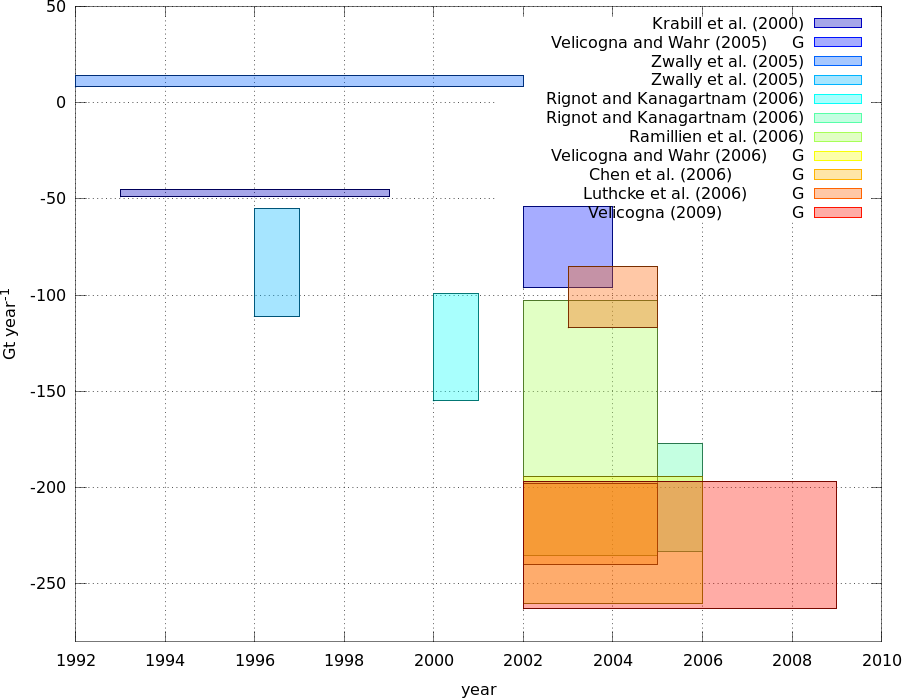
\includegraphics[width=0.55\textwidth]{greenlandboxes}
\end{center}

\vspace{-0.21in}
\item context:\footnote{Gt = gigatonne $\approx \text{km}^3$}
  \begin{itemize}
  \item[$\circ$]  Greenland ice sheet mass is $2.7 \times 10^9$ Gt % = 2.93466 10^6 km^3  volume, from SeaRISE-Greenland 5km data
  \item[$\circ$]  if \emph{all} Greenland ice melts then we get 7 m of sea level rise
  \item[$\circ$]  if \emph{all} Antarctic ice melts then we get 61 m
  \end{itemize}
\end{itemize}
\end{frame}


\section[shallow ice approximation]{shallow ice approximation for grounded ice sheets}


\begin{frame}
  \frametitle{the main variables}

\begin{center}
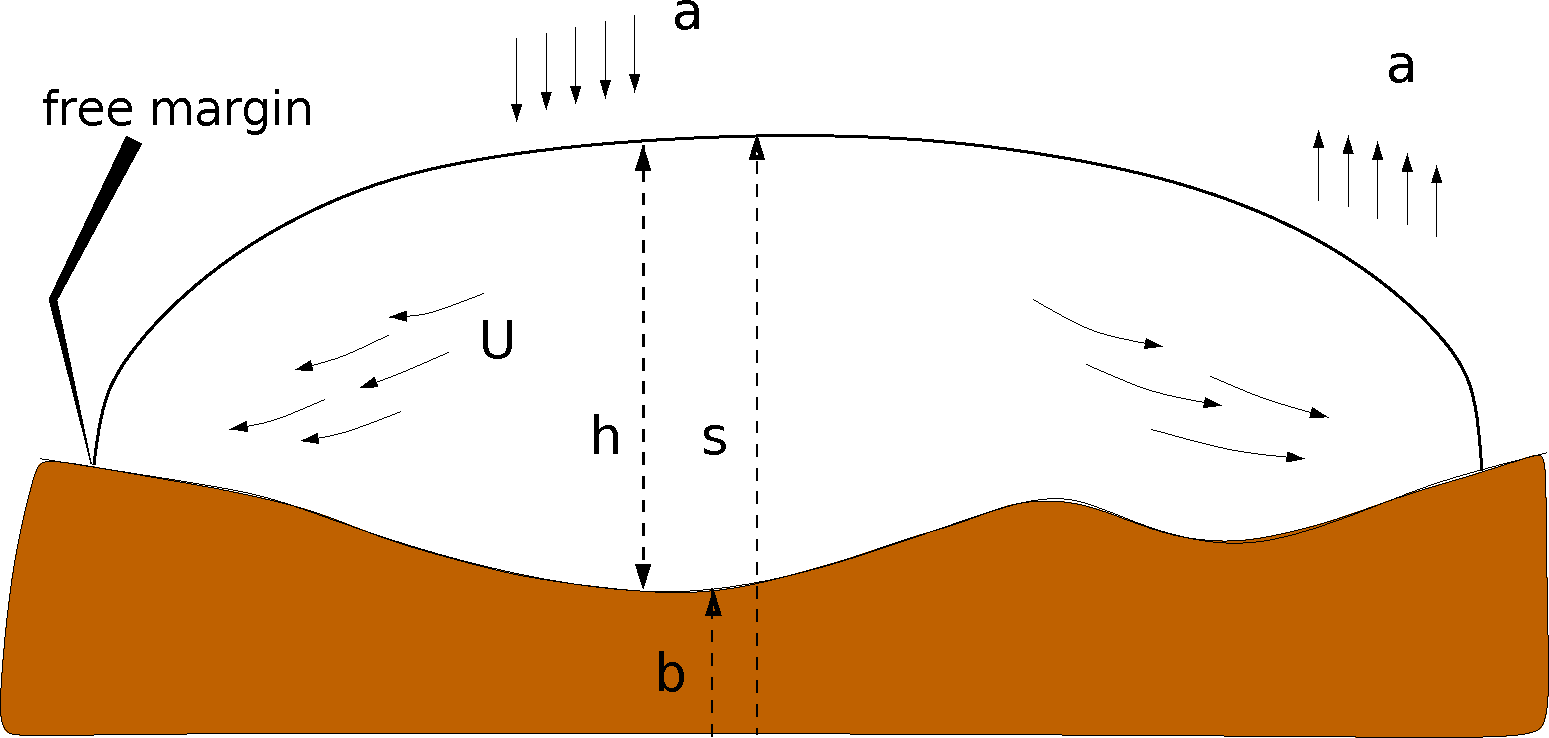
\includegraphics[width=0.7\textwidth]{groundedscheme}
\end{center}

\begin{itemize}
\small
\item $b(x,y)=$ bedrock elevation
\item $s(t,x,y)=$ ice surface elevation
\item $h(t,x,y)=$ ice thickness $ = s-b$
\item ${\bf U}(t,x,y,z)=$ horizontal velocity field
\item $a(t,x,y,z)=$ yearly-average mass balance \onslide<2>{\color{dark green} [Ed: explain m.b.]}
\end{itemize}

\begin{alertblock}<3>{key idea: ice surface $s$ is always above the bedrock $b$}
\end{alertblock}
\end{frame}


\begin{frame}
  \frametitle{shallow ice approximation (SIA)}

\begin{itemize}
\item SIA = lubrication approximation of Stokes model
\item good approximation when:
  \begin{itemize}
  \item[$\circ$] sliding is small or zero
  \item[$\circ$] bedrock slope is modest
  \end{itemize}
\item derive SIA equations by scaling Stokes:
  \begin{itemize}
  \item[$\circ$] $[h]$ is a typical thickness scale
  \item[$\circ$] $[x]$ is a typical width scale
  \item[$\circ$] small parameter is $\eps = [h] / [x]$
  \end{itemize}
\item for this part of the talk: consider only grounded ice sheets
  \begin{itemize}
  \item[$\circ$] so $h \to 0$ continuously at margin
  \item[$\circ$] i.e.~\emph{not} marine ice sheets
  \end{itemize}
\end{itemize}
\end{frame}


\begin{frame}
  \frametitle{SIA: velocity}
 
\begin{itemize}
\item let $p=n+1>2$
\item assume: no sliding and isothermal
\item horizontal ice velocity is given by: 
  $${\bf U}  =  - \frac{2 A}{p} (\rho g)^{p-1} \left[ (s-b)^p - (s - z)^p  \right] 
|\nabla s |^{p-2} \nabla s$$
\item no PDE needs to be solved to compute velocity!
\end{itemize}
\end{frame}


\begin{frame}
  \frametitle{SIA: steady state}

\begin{itemize}
\item mass conservation in steady state: 
  $$\Div \left(  \int_b^s {\bf U}\, dz \right)  =  a$$
\item shallow ice approximation + (steady) mass conservation:
  $$- \Div \left(\Gamma (s-b)^{p+1} | \nabla s |^{p-2} \nabla s  \right) =  a$$
  \begin{itemize}
  \vspace{-0.2in}
  \item[$\circ$] this is the major SIA equation (\dots a PDE?)
  \item[$\circ$] computes ice surface $s$
  \item[$\circ$] constant $\Gamma > 0$ combines $\rho,g,A,p$
  \item[$\circ$] $p$-Laplacish \dots but coefficient $(s-b)^{p+1} \to 0$ at margins
  \end{itemize}
\end{itemize}
\end{frame}


\begin{frame}{time-dependent SIA}

\begin{columns}
\begin{column}{0.4\textwidth}
\small
\begin{itemize}
\item instead of formulas, show a similarity solution
\item at right is the Halfar (1981) solution, an exact, time-dependent, zero mass balance solution where the $t\to 0^+$ limit is a delta function
\item compare Barenblatt solution of porous medium equation
\end{itemize}
\end{column}

\begin{column}{0.65\textwidth}
\vspace{-0.25in}

\begin{center}
\animategraphics[autoplay,loop,height=4.7cm]{4}{../GGseminar12/anim/halfar}{0}{26}

\bigskip
\tiny
frames from $t=4$ months to $t = 10^6$ years,

equal spaced in \emph{exponential} time
\end{center}
\end{column}
\end{columns}
\end{frame}


\begin{frame}
  \frametitle{a change of variable}
 
\begin{itemize}
\item using the change of variable  $u=h^{ \frac{2p}{p-1}}$, the steady SIA equation is:
\begin{empheq}[]{equation*}
 -  \Div \left( \mu  | \nabla u - \Phi(u) |^{p-2}
  ( \nabla u - \Phi(u) )  \right)  = \alpha(u)
\end{empheq}

where
  \begin{itemize}
  \item[$\circ$]  $\mu>0$ is constant (isothermal case)
  \item[$\circ$]  $\Phi(u) = - C \, u^{\frac{p+1}{2p}} \nabla b$ is transformed bedrock topography
  \item[$\circ$]  $\alpha(u) = a(x,y,z\!=\!u^{\frac{p-1}{2p}} )$ is transformed mass balance
  \end{itemize}
\item a generalized $p$-Laplace equation with added nonlinearities
\item change of vars means uniform $p$-ellipticity recovered (i.e.~$\mu>0$) but at cost of ``tilt'' ($\nabla u - \Phi(u)$)
\end{itemize}
\end{frame}


\begin{frame}
  \frametitle{SIA: weak formulation = variational inequality} 

\begin{itemize}
\item issue: SIA equation applies only on domain where $s>b \iff h > 0$
\item the change $h \to u$ transforms  constraint $s \ge b$ into $u \ge 0$
\item define convex constraint set
  $$\Kcal := \{ v \in W^{1,p}_0 (\Omega), v \ge 0 \}$$
\end{itemize}

\begin{block}{definition} 
$u \in \Kcal$ solves the \emph{steady shallow ice sheet problem} if
\begin{align*}
\int_{\Omega}    \left( \mu  | \nabla u - \Phi(u) |^{p-2} 
( \nabla u - \Phi(u) )    \right)  \cdot \nabla ( v - u )  
\ge \int_{\Omega} \alpha(u) (  v -  u ) 
\end{align*}
for all $v \in \Kcal$ \hfill \scriptsize (Jouvet-Bueler 2012)
\end{block}
\end{frame}


\begin{frame}
  \frametitle{SIA: an analogy}

\begin{columns}
\begin{column}{0.35\textwidth}
\begin{itemize}
\item ice sheet surface \\ = \alert{membrane}
\item bedrock = \alert{obstacle}
\end{itemize}
\vfill
\begin{center}
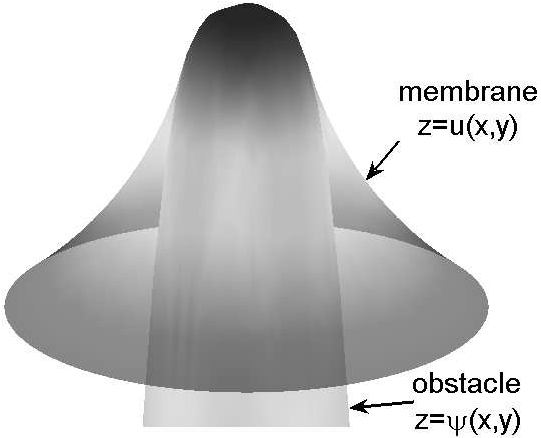
\includegraphics[width=1.1\textwidth]{classicalobs}
\end{center}
\end{column}
\begin{column}{0.65\textwidth}
\begin{center}
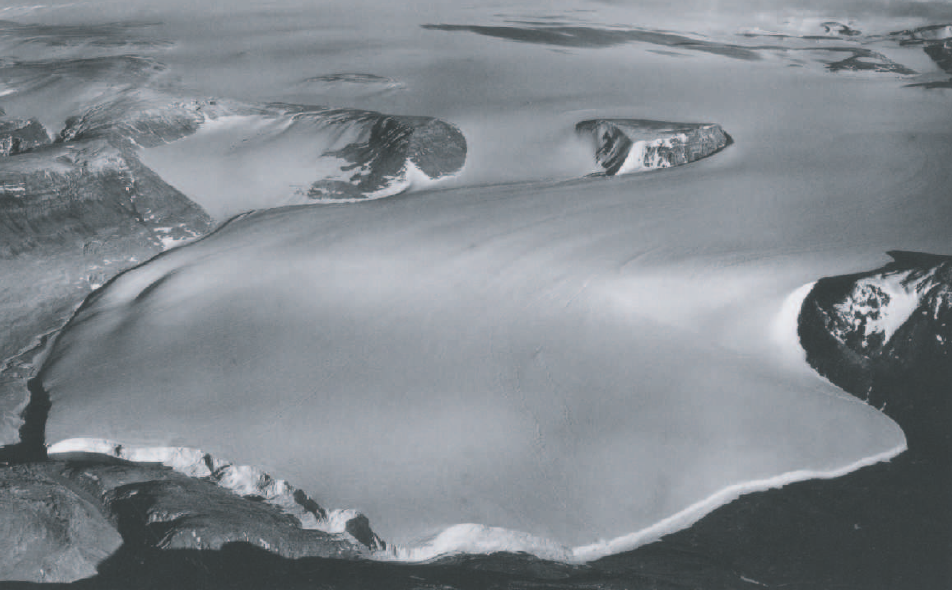
\includegraphics[width=0.8\textwidth]{polaris} \\
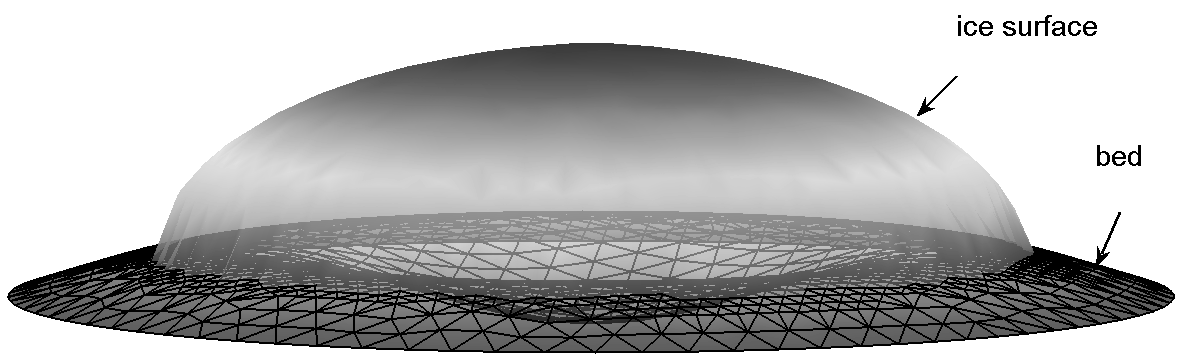
\includegraphics[width=\textwidth]{capnonflatobs}
\end{center}
\end{column}
\end{columns}
\end{frame}


\begin{frame}
  \frametitle{existence and uniqueness for a restricted problem} 

\begin{block}{(easy) theorem}
if $\alpha,\Phi$ were independent of $u$ then the variational inequality is equivalent to:

\begin{equation*}
u \text{ minimizes} \qquad J(v) = \frac{\mu}{p} \int_{\Omega} |\nabla v - \Phi |^p - \int_{\Omega}  \alpha v
\end{equation*}

over $v\in\mathcal{K}$; this admits a unique solution \hfill \scriptsize (Jouvet-Bueler 2012)
\end{block}

\bigskip
\begin{itemize}
\item gives ice sheet existence and uniqueness only if
  \begin{itemize}
  \item[$\circ$]  bedrock is flat ($\Phi = 0$) and
  \item[$\circ$]  mass balance is elevation-independent ($a=a(x,y)$)
  \end{itemize}
\item but otherwise: $\alpha,\Phi$ are not independent of $u$
\end{itemize}
\end{frame}
 

\begin{frame} 
  \frametitle{ existence in the general case } 

\begin{itemize}
\item $p>2$ so $W^{1,p}_0 (\Omega) \hookrightarrow C(\overline{\Omega})$
\item define map $\mathcal{A}:C(\overline{\Omega}) \rightarrow C(\overline{\Omega})$,
which takes $w$ to the unique $u$ solving (over $v\in \mathcal{K}$)
\begin{align*}
\int_{\Omega}   \mu  \left( | \nabla u - \Phi(w) |^{p-2} 
( \nabla u - \Phi(w) )    \right)  \cdot \nabla ( v - u )  
\ge \int_{\Omega} \alpha(w) (  v -  u )
\end{align*}
\end{itemize}

\begin{block}{result}
the map $\mathcal{A}$ admits at least one fixed point \hfill \scriptsize (Jouvet-Bueler 2012)
\end{block}

\vfill
\scriptsize
sketch of proof:
\begin{itemize}
\item $\mathcal{A}$ is continuous and compact
\item the set $\{ w \in C(\overline{\Omega}), \exists \lambda \in [0,1]\, \text{so that} \,w = \lambda \mathcal{A}(w)\}$ is bounded 
\item Schaefer's fixed point theorem
\end{itemize}
\end{frame}


\begin{frame}
  \frametitle{thus: fixed-point iteration on variational inequality} 

\begin{itemize}
\item given bedrock topography $b(x,y)$
\item given mass-balance $a(x,y)$ (steady climate)
\item set $u_0 = 0$
\item do fixed point iterations for $u_{k+1} \in \mathcal{K}$:
\begin{align*}
\int_{\Omega} &\left( \mu |\nabla u_{k+1} - \Phi(u_k)|^{p-2}
(\nabla u_{k+1} - \Phi(u_k) ) \right) \cdot \nabla (v - u_{k+1}) \\
&\qquad\qquad \ge \int_{\Omega} \alpha (v -  u_{k+1})
\end{align*}

\bigskip
\item \emph{computes}: steady state ice sheet shape
\end{itemize}
\end{frame}


\begin{frame}
  \frametitle{example: steady ice sheet on Greenland bedrock}

\begin{itemize}
\item first iterations from zero ice:

\begin{center}
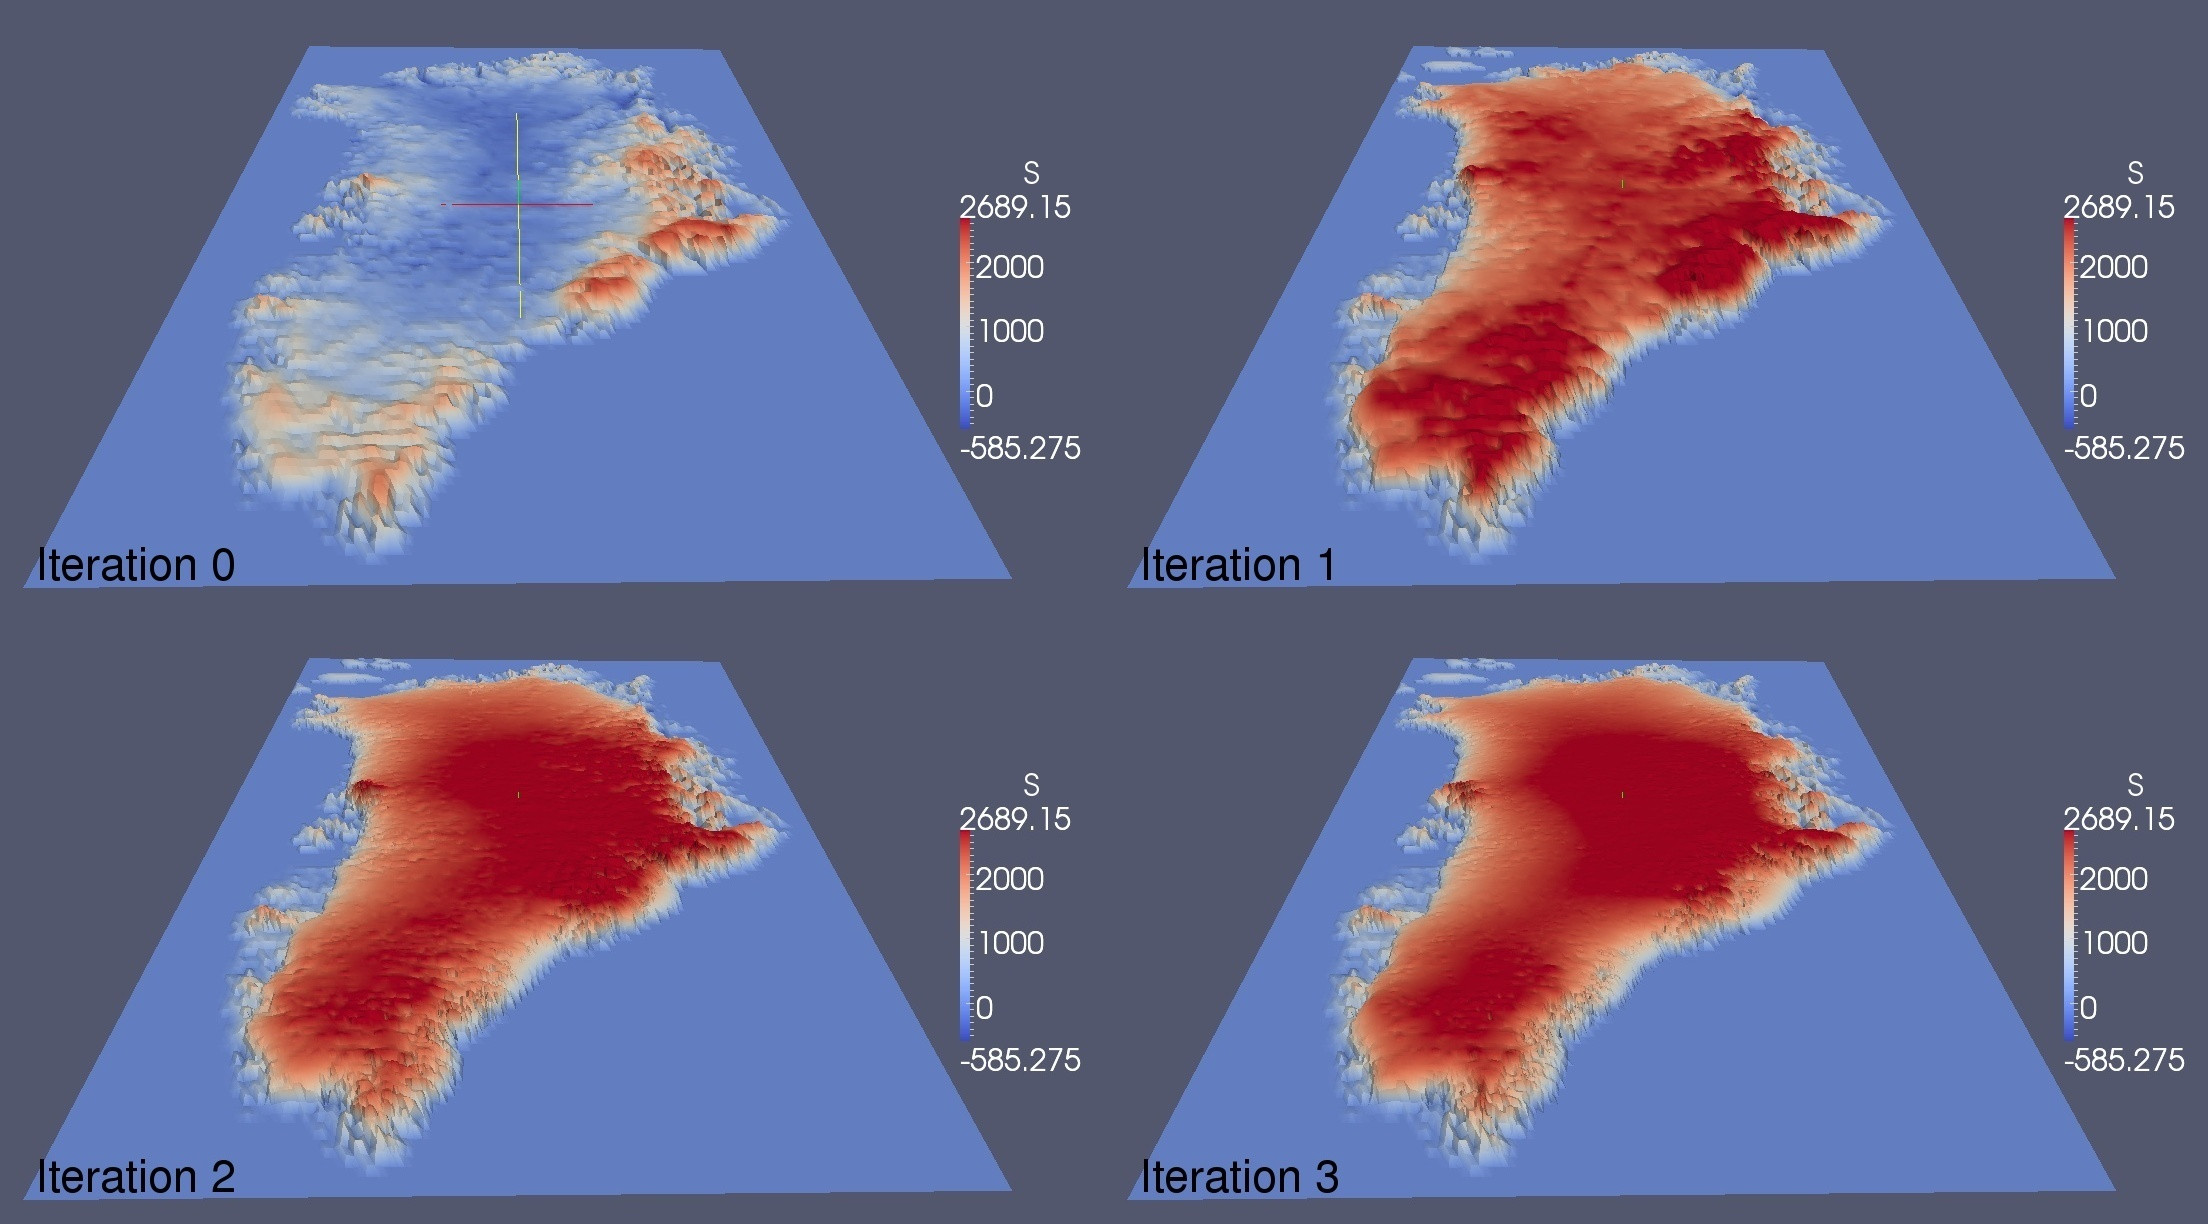
\includegraphics[width=0.9\textwidth]{greenland-result.jpg}
\end{center}
\item as far as we can tell: this 2011 computation was the first of the steady state of a real ice sheet \emph{without} time-stepping
\end{itemize}
\end{frame}


\begin{frame}
  \frametitle{quality of this variational inequality} 

\begin{itemize}
\item every glaciologist believes this about steady climates:
	$$\text{if } a > 0 \text{ on a sub-domain } R \text{ then } s > b \text{ on } R$$
\item that is:
\begin{center}
 if it snows more than it melts then you get a glacier there
\end{center}
\end{itemize}

\begin{columns}
\begin{column}{0.6\textwidth}
\begin{itemize}
\small
\item uniformly-elliptic variational inequalities, e.g.~the classical obstacle problem,
\begin{align*}
\int_{\Omega}  \nabla u \cdot \nabla (v - u)  \ge  \int_{\Omega} f (v - u),
\end{align*}
for all $v\ge \psi$, do \emph{not} have the analogous property
\end{itemize}
\end{column}
\begin{column}{0.4\textwidth}
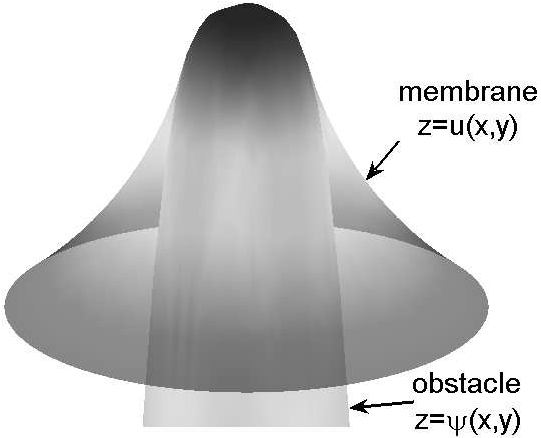
\includegraphics[width=\textwidth]{classicalobs}
\end{column}
\end{columns}
\end{frame}


\section[ice streams]{a model for ice streaming}


\begin{frame}
  \frametitle{shallow shelf approximation (SSA): a ``definition''}

\begin{columns}
\begin{column}{0.52\textwidth}
\begin{itemize}
\small
\item SSA = ``membrane'' or ``plug'' flow approximation of Stokes
\item a good approximation when there is low basal resistance and minimal basal topography
\item a very good approximation for ice shelves (next slide)
\item derived by scaling with $\eps = [h]/[x]$ \emph{and} requirement that basal resistance is low (see Schoof (2006))
\end{itemize}
\end{column}

\begin{column}{0.48\textwidth}
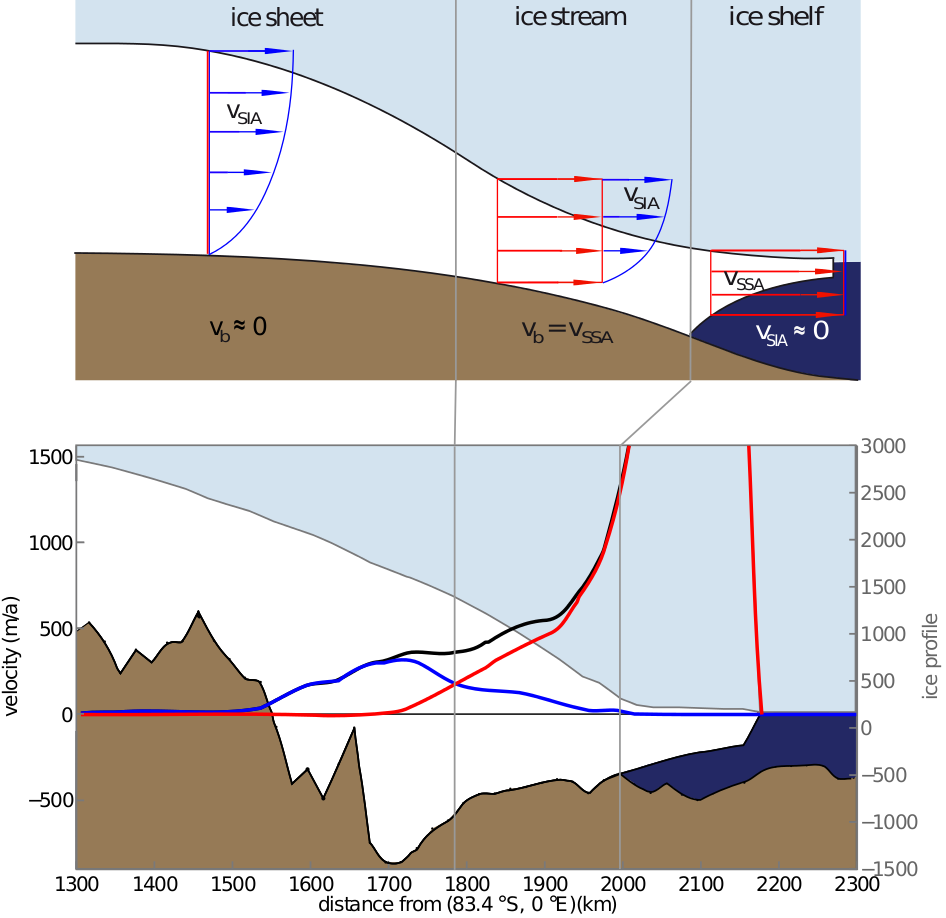
\includegraphics[width=1.1\textwidth]{siassacartoon-lambert}

\begin{center}
\vspace{-0.18in}
\tiny [Lambert glacier and Amery ice shelf, Antarctic]
\end{center}
\end{column}
\end{columns}
\end{frame}


\begin{frame}{SSA works \emph{well} for ice shelves}

\begin{itemize}
\item Ross ice shelf (Antarctica) velocity below
  \begin{itemize}
  \item[$\circ$] observed versus computed by SSA model in PISM
  \item[$\circ$] tuned: single, constant $A$
  \end{itemize}
\end{itemize}
\vspace{-0.3in}

\begin{center}
  \mbox{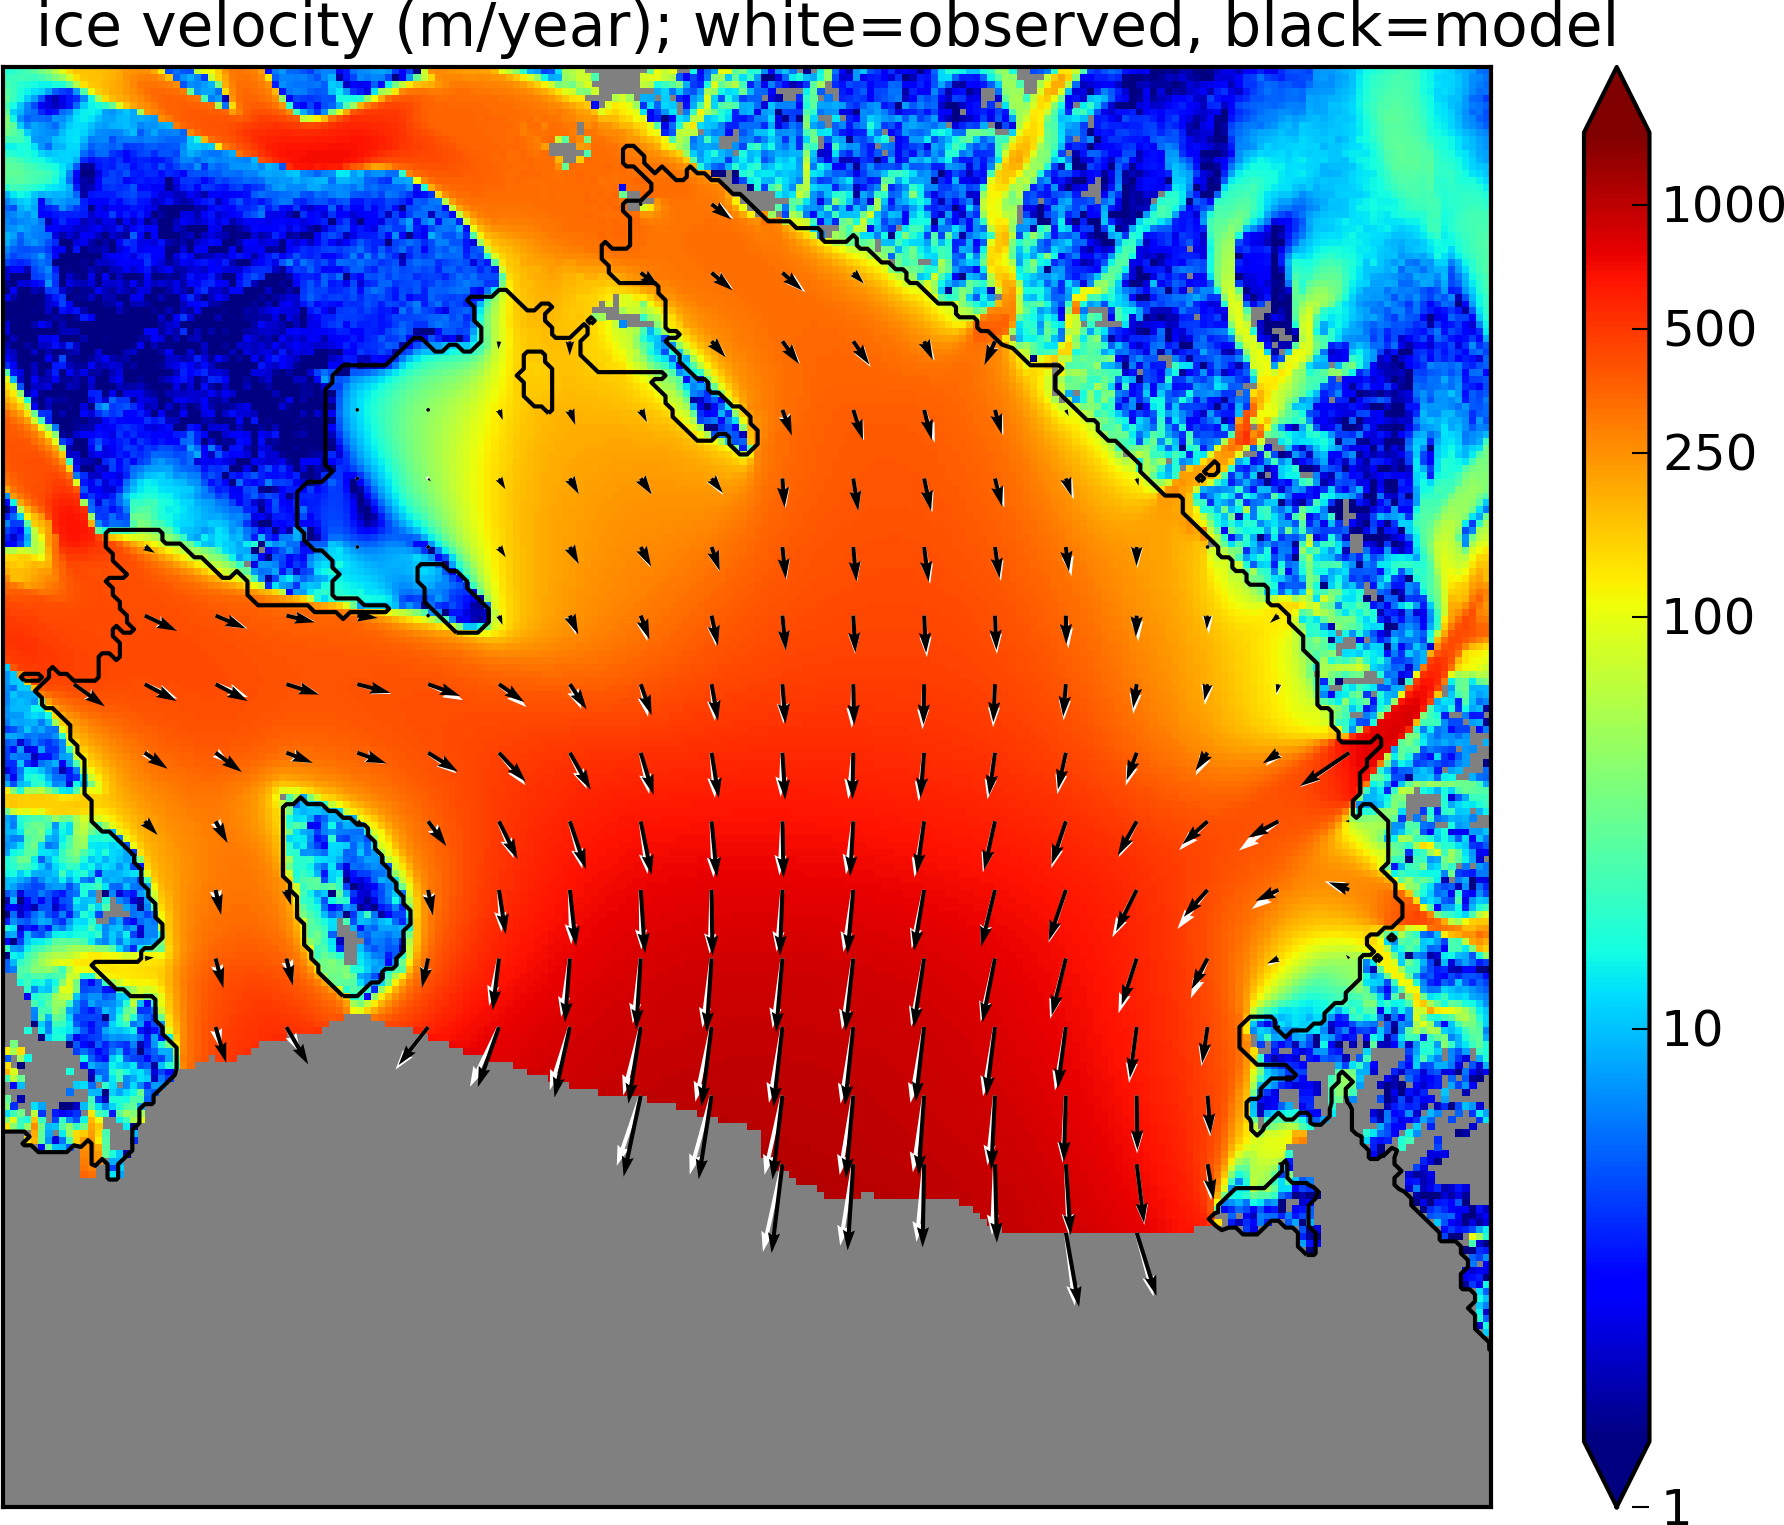
\includegraphics[width=0.58\textwidth]{rossquiver} \, 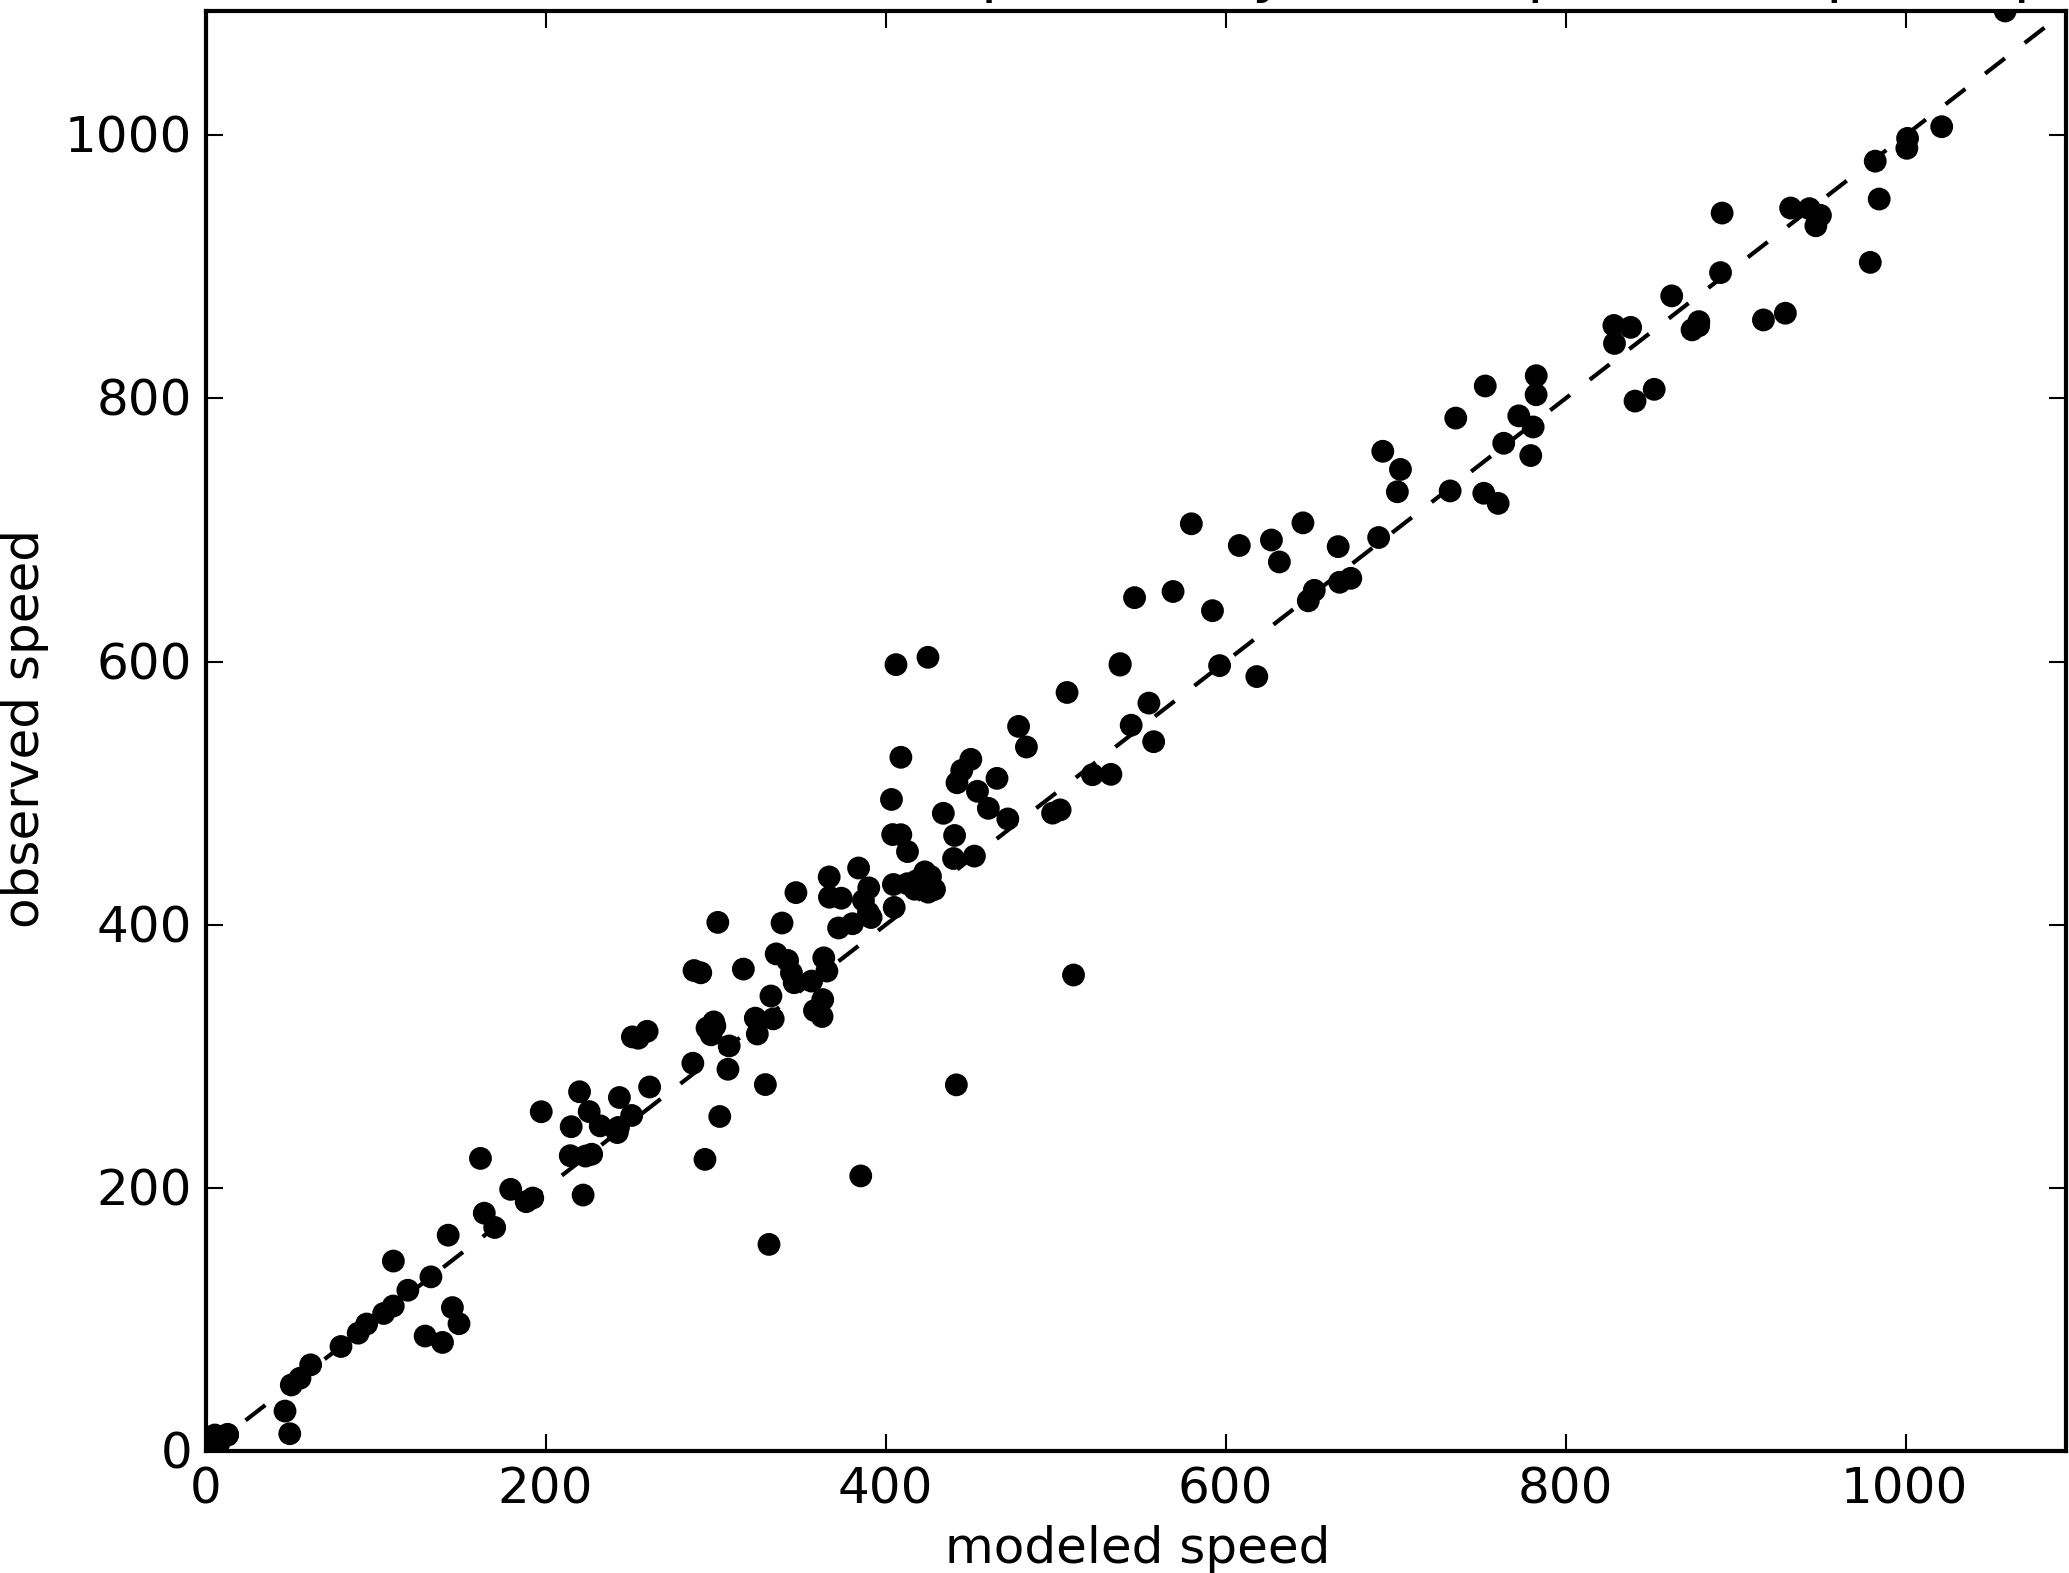
\includegraphics[width=0.48\textwidth]{rossscatter}}
\end{center}
\end{frame}


\begin{frame}
  \frametitle{SSA for ice streams: an analogy}

\begin{columns}
\begin{column}{0.6\textwidth}
\begin{itemize}
\item ice shelves have zero basal resistance
\item ice streams emerge where basal resistance is sufficiently low

(\emph{top}: Siple coast ice streams)
\item a basal resistance model:
  \begin{itemize}
  \item[$\circ$] ``plastic'' or Coulomb friction 
  \item[$\circ$] distribution of yield stress $\tau_c$
  \end{itemize}
\item ice membrane connects to upstream and/or lateral high friction with viscous stresses (\emph{bottom}: Schoof's slider analogy)
\end{itemize}
\end{column}
\begin{column}{0.4\textwidth}
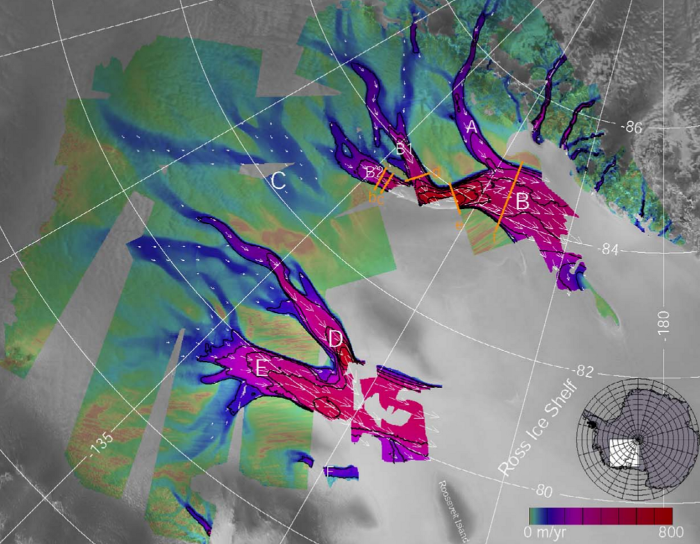
\includegraphics[width=\textwidth]{siple}

\vspace{0.3in}

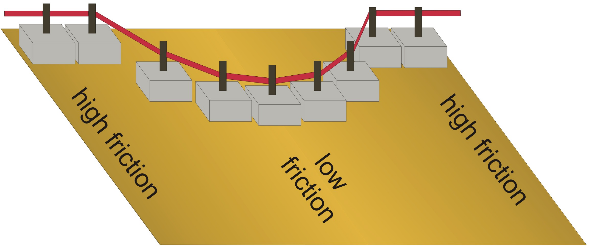
\includegraphics[width=1.1\textwidth]{schoof-sliders}
\end{column}
\end{columns}
\end{frame}


\begin{frame}
  \frametitle{SSA weak formulation}

\begin{itemize}
\item let $q = 1+\frac{1}{n}$ and $B = A^{1-q}$
\item suppose a basal yield stress distribution $\tau_c(x,y)$, zero on ice shelves
\item $2\,\Tnorm{\mathbf{V}}^2 := \sum_{i,j} (\mathbf{D}V_{ij})^2 + \sum_{i} (\mathbf{D}V_{ii})^2$
\item $\mathbf{F}$ is lateral force along calving front
\end{itemize}

\begin{block}{definition}
the horizontal velocity $\mathbf{U}\in W^{1,q}(\Omega)$ solves the SSA if it minimizes
\small
\begin{align*}
\mathcal{J}_{\text{SSA}}(\mathbf{V}) &= \int_\Omega \frac{2 B}{q} h \Tnorm{\mathbf{V}}^q + \rho g h \grad s \cdot \mathbf{V} + \tau_c |\mathbf{V}| + \int_{\partial\Omega} \mathbf{F} \cdot \mathbf{V}
\end{align*}
\end{block}

\normalsize
\begin{itemize}
\item because $\mathcal{J}_{\text{SSA}}$ is not differentiable (``$\tau_c |\mathbf{V}|$''), minimization is equivalent to variational inequality
\end{itemize}
\end{frame}


\begin{frame}
  \frametitle{SIA+SSA hybrid velocity model}

\begin{itemize}
\item FIXME:
\end{itemize}
\end{frame}


\section[marine ice sheets]{a model for marine ice sheet evolution}

\begin{frame}
  \frametitle{marine ice sheets: setting}

\begin{itemize}
\item marine ice sheets have all modes of flow
\item full of free boundaries
\item there is only one marine ice sheet:  Antarctic ice sheet
\end{itemize}

\begin{center}
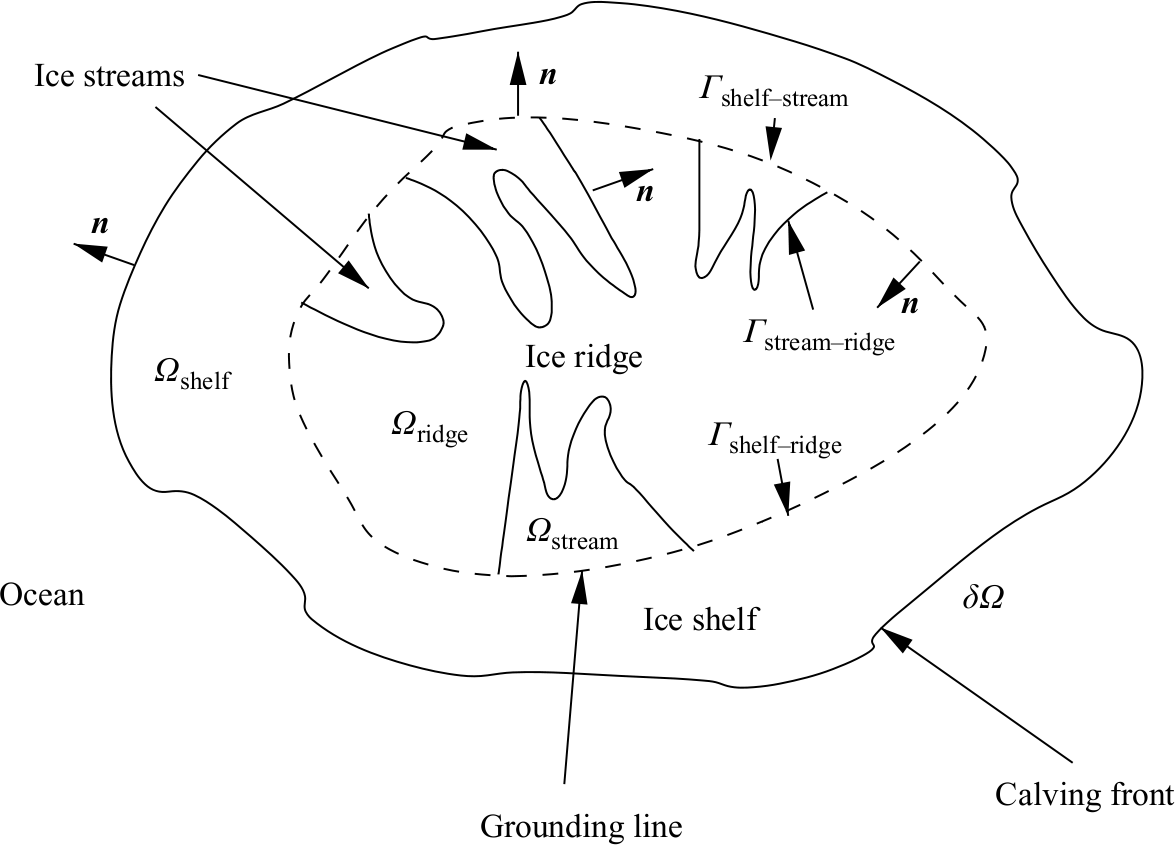
\includegraphics[width=0.7\textwidth]{schoof-planform}

\tiny figure from (Schoof, 2006)
\end{center}
\end{frame}


\begin{frame}
  \frametitle{setting marine ice sheet evolution}

\begin{itemize}
\item $x$ is a point in the map-plane (i.e.~$(x,y)$)
\item $t_0,t_1,\dots,t_K$ is time-discretization with spacing $\tau_k = t_{k+1}-t_k$
\item recall $p = n+1$ and $q = 1 + \frac{1}{n}$ and $n\approx 3$
\end{itemize}
\end{frame}


\begin{frame}
  \frametitle{an algorithm for marine ice sheet evolution}


\begin{enumerate}
\small
\item find velocity $\mathbf{U}_k \in \Wq$ that minimizes
\begin{align*}
\mathcal{J}_{\text{SSA}}(\mathbf{V}) &= \frac{2 A^{1-q}}{q} \int_\Omega h_k \Tnorm{\mathbf{V}}^q + \rho g h_k \grad s_k \cdot \mathbf{V} \\
  &\qquad\qquad + \int_{G(h_k)} \tau_c |\mathbf{V}| + \int_{\partial\Omega} \mathbf{F}_k \cdot \mathbf{V}
\end{align*}
\item find $h_{k+\frac12}$, the solution at $t_{k+1}$ of the advection problem:
$$\begin{cases}
  \frac{\partial h}{\partial t} + \Div \left(\mathbf{U}_k\, h\right) = 0, & t_k \le t \le t_{k+1}, \\
  h(t_k) = h_k. &
\end{cases}$$
\item find thickness $h_{k+1} = u^{\frac{p-1}{2p}}$, i.e.~find $u\in\mathcal{K}$, that minimizes  % $u=h^{ \frac{2p}{p-1}}$
\begin{align*}
\mathcal{J}_{\text{SIA}}(v) &= \frac{1}{2 \tau_k} \int_\Omega v^2 + FIXME
\end{align*}
\end{enumerate}
\end{frame}


\begin{frame}
  \frametitle{an algorithm for marine ice sheet evolution}

some concerns:
\begin{itemize}
\item 
\end{itemize}
\end{frame}


\begin{frame}
  \frametitle{FEM solution of var ineq}

\begin{itemize}
\item FIXME: TNNMG
\end{itemize}
\end{frame}


\begin{frame}
  \frametitle{moving grounding line}

FIXME: model is SIA+SSA with adaptive grid

\begin{center}
\PDFAnimation{exp3a}
\end{center}
\end{frame}


\begin{frame}
  \frametitle{mundane}

\begin{itemize}
\item FIXME: PISM results for Greenland and Antarctica
\end{itemize}
\end{frame}


\section*{conclusion}

\begin{frame}
  \frametitle{conclusion: some new thinking which is weak and shallow}

\begin{itemize}
\item work on steady states (walk before fly)
\item steady grounded ice sheets now have a well-posed obstacle-like formulation (a $p>2$-Laplace variational inequality for SIA+mass)
\item sliding ice sheets have a theory in which ice streams ``emerge naturally'' (a $p<2$-Laplace variational inequality for SSA)
\item marine ice sheet paradigm from time-splitting:
  \begin{itemize}
  \item[$\circ$]  solve SSA problem
  \item[$\circ$]  advection with SSA velocity
  \item[$\circ$]  solve SIA+mass obstacle problem
  \end{itemize}
\end{itemize}
\end{frame}


%%%%%%%%%%%%%%

% EXTRA SLIDES

\begin{frame}
  \frametitle{full and simplified (shallow) ice flow models }

\begin{center}
\begin{tabular}{|c|c|c|}
\hline name & unknowns  & equation (+incompressibility)   \\ 
\hline Stokes & 
$\left(
\begin{array}{c}
u \\ 
v \\ 
w  
\end{array} \right),p$ &  
$  \nabla \cdot \left(
\begin{array}{ccc}
\tau_{xx} & \tau_{xy} & \tau_{xz} \\ 
\tau_{yx} & \tau_{yy} & \tau_{yz} \\ 
\tau_{zx} & \tau_{zy} & \tau_{zz}  
\end{array} \right) = \left(
\begin{array}{c}
0 \\ 
0 \\ 
\rho g  
\end{array} \right)$  \\ 
\hline B.-P.\footnote{\tiny Blatter-Pattyn approximation} & 
$\left(
\begin{array}{c}
u \\ 
v 
\end{array} \right) $  & 
$ \nabla \cdot \left(
\begin{array}{ccc}
\tau_{xx} & \tau_{xy} & \tau_{xz} \\ 
\tau_{yx} & \tau_{yy} & \tau_{yz} \\ 
0 & 0 & \tau_{zz}  
\end{array} \right) = \left(
\begin{array}{c}
0 \\ 
0 \\ 
\rho g  
\end{array} \right)$  \\  
\hline SSA\footnote{\tiny shallow shelf approximation} &
$ \left(
\begin{array}{c}
u \\ 
v  
\end{array} \right) $ & 
$ \nabla \cdot \left(
\begin{array}{ccc}
\tau_{xx} & \tau_{xy} & 0 \\ 
\tau_{yx} & \tau_{yy} & 0 \\ 
0 & 0 & \tau_{zz}  
\end{array} \right) = \left(
\begin{array}{c}
0 \\ 
0 \\ 
\rho g  
\end{array} \right)$ \\ 
\hline SIA\footnote{\tiny shallow ice approximation} & $\emptyset$ &
$ \nabla \cdot \left(
\begin{array}{ccc}
0 & 0 & \tau_{xz} \\ 
0 & 0 & \tau_{yz} \\ 
0 & 0 & \tau_{zz}  
\end{array} \right) = \left(
\begin{array}{c}
\rho g \frac{\partial s}{\partial x}\\ 
\rho g \frac{\partial s}{\partial y} \\ 
\rho g  
\end{array} \right)$ \\ 
\hline 
\end{tabular}  
\end{center}
  
\end{frame}


\end{document}

